\section{Introduction}
\begin{figure}[!h]
% \vspace{-2mm}
\centering
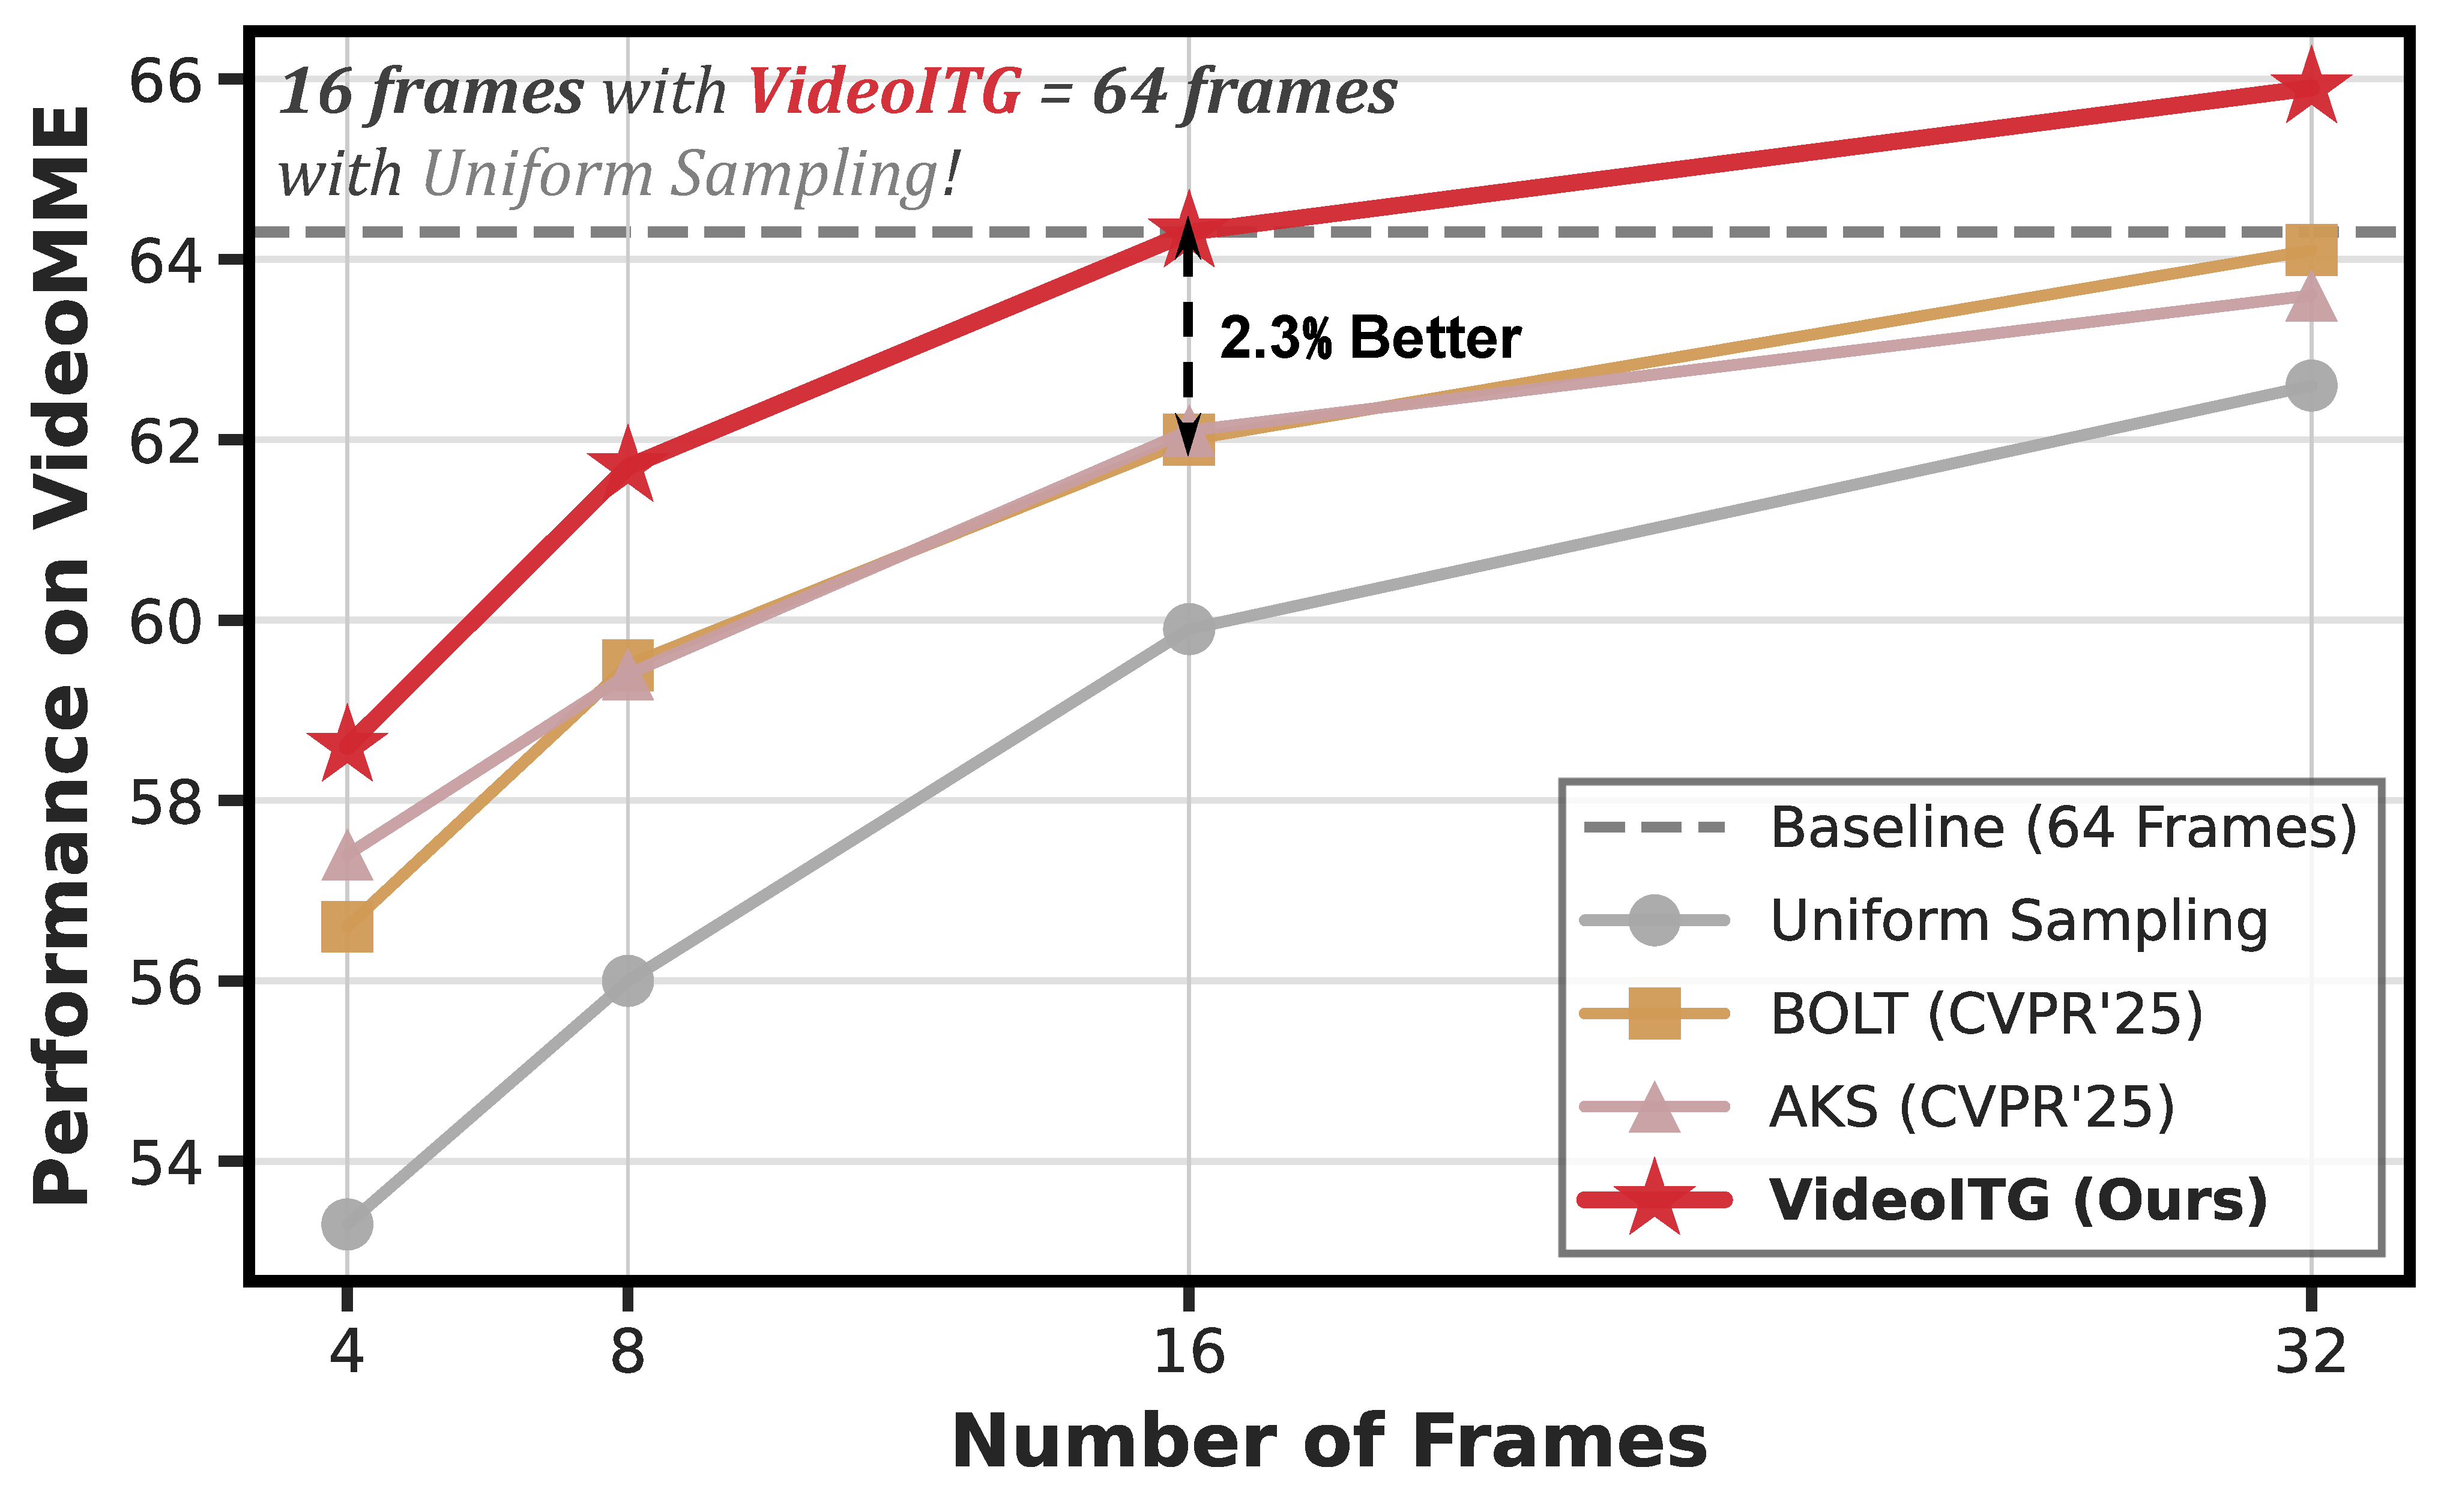
\includegraphics[width=0.95\linewidth]{frames.pdf}
\vspace{-3mm}
\caption{\noindent \textbf{Comparison of different frame selection methods on VideoMME with LLaVA-Video-7B.} VideoITG consistently enhances baseline methods and achieves state-of-the-art performance.}
\label{fig:frames}
\vspace{-2mm}
\end{figure}
The rapid progress of Video Large Language Models (Video-LLMs) has opened new frontiers in video understanding, enabling complex tasks such as captioning~\cite{chensharegpt4video, chai2025auroracap, zhou2024streaming, islam2024video, chen2024large, wang2024tarsier}, visual question answering~\cite{bai2025qwen3, fu2024videomme, zhou2024mlvu, mangalam2024egoschema, li2024mvbench, chen2024cg, xiao2021next, patraucean2023perception}, and even embodied-agent interaction~\cite{brohan2023rt, kim2024openvla, fu2024vita, liu2024streamchat, chen2024videollm, chen2025grounded}. 
However, these models still struggle with long videos, where high memory cost and computation overhead limit their ability to process extended temporal contexts. 
A common workaround is uniform frame sampling—simple yet suboptimal—often missing key frames critical for semantic and temporal reasoning, thereby constraining overall performance.

To alleviate this challenge, prior studies have explored multiple directions. 
One class of approaches focuses on reducing spatiotemporal redundancy through pooling~\cite{xu2024pllava, shen2024longvu}, similarity pruning~\cite{zhang2024flash}, or clustering-based compression~\cite{li2024llavaonevision, zhang2024internlm}, retaining only essential frames. 
Another line extends model sequence length to capture long-term dependencies~\cite{wang2024qwen2, team2023gemini}, yet such strategies incur high computation and risk information dilution. 
Other methods incorporate question-centric cues for frame selection~\cite{li2024llama, yu2023self}, demonstrating superiority over uniform sampling (\ref{fig:frames}). 
For example, SeViLA~\cite{yu2023self} applies BLIP-2~\cite{li2023blip} to process each frame independently before selecting keyframes, which are then fed into video reasoning pipelines. 
Nevertheless, the absence of temporal modeling across frames hinders effective reasoning over multi-event or time-sensitive queries.

\begin{figure*}[t!]
\centering
\vspace{-1mm}

\includegraphics[width=0.92\linewidth]{intro.pdf}
\vspace{-2mm}
\caption{
\textbf{Overview of the \textit{VidThinker} annotation pipeline for VideoITG.}
It consists of three human-inspired stages: (1) clip-level captioning under instructions; (2) instruction-guided relevant clip retrieval; and (3) fine-grained frame-level localization.
}
\label{intro}
\vspace{-4mm}
\end{figure*}

Despite progress in compressing or extending temporal contexts, a substantial performance gap remains between short and long videos—primarily due to the lack of large-scale, instruction-guided temporal grounding data. 
When humans analyze long videos, they rarely process all frames at once; instead, they skim for global context, identify question-relevant cues, and zoom in on discriminative moments. 
Inspired by this human strategy, we propose \textbf{Instructed Temporal Grounding for Videos (VideoITG)}, which integrates user instructions directly into the frame selection process. 
While traditional temporal grounding~\cite{wang2024grounded, qian2024momentor, lei2021detecting} focuses on localizing events using single descriptive queries, \textbf{VideoITG} introduces instruction-driven temporal reasoning, adaptively customizing the sampling strategy for each task. 
Unlike prior frame selection frameworks~\cite{yu2023self, yu2025frame, han2025videoespresso, meng2022adavit, wang2022efficient}, 
our method handles multi-temporal and multi-cue scenarios by (i) localizing temporal cues across clips for relational reasoning, (ii) employing hybrid sampling for dynamic event variations, and (iii) maintaining holistic coverage for content verification and captioning.

To support VideoITG, we construct a large-scale dataset via an automated annotation pipeline named \textit{VidThinker}. 
As shown in Fig.~\ref{intro}, VidThinker automates data generation through instruction-conditioned clip captioning, instruction-guided retrieval, and fine-grained frame localization. 
Driven by GPT-4o~\cite{openai2024gpt4o} reasoning, VidThinker emulates a "Needle-in-a-Haystack" process to retrieve relevant moments and provides balanced supervision across four instruction types: 
\textbf{(1) semantic-only}, focusing on appearance; 
\textbf{(2) motion-only}, emphasizing dynamic cues; 
\textbf{(3) semantic \& motion}, for joint reasoning; and 
\textbf{(4) non-clues}, open-ended video-level prompts that require maximizing visual diversity across the entire video.

The resulting \textbf{VideoITG-40K} dataset contains 40K videos (30s–3min) and 500K instruction-grounded annotations—surpassing existing temporal grounding datasets by more than \textbf{4$\times$} in both scale and instruction quality. 
Building on this foundation, we design a family of VideoITG models—featuring text generation, anchor-based causal attention, and full-attention pooling—to effectively align temporal cues with user instructions. 

In summary, our key contributions are as follows:
\begin{itemize}[leftmargin=6mm, itemsep=3pt, parsep=0pt, topsep=2pt]
    \item \textbf{VideoITG-40K dataset.} 
    Built via the automated \textit{VidThinker} pipeline, we curate \textbf{VideoITG-40K}, it contains 40K videos and 500K fine-grained, instruction-aligned annotations, substantially expanding the scale and diversity of existing temporal grounding resources.
    \item \textbf{VideoITG models.} 
    We propose three complementary model variants that explore distinct attention and decoding mechanisms, offering a unified, plug-and-play framework adaptable to diverse Video-LLMs.
    \item \textbf{Consistent improvement.} 
    Across benchmarks and models, VideoITG boosts accuracy with fewer frames: on VideoMME (Fig.~\ref{fig:frames}), 16 frames with VideoITG match 64-frame uniform sampling and are comparable to SOTA methods using 32 frames.
\end{itemize}
